\input{defs}
\section{Introduction}
Large language model (LLM) agents are increasingly deployed in multi-turn, tool-grounded environments such as customer support~\citep{yao2024taubenchbenchmarktoolagentuserinteraction}, web navigation~\citep{zhou2024webarenarealisticwebenvironment, drouin2024workarenacapablewebagents, lu2025toolsandboxstatefulconversationalinteractive}, and software engineering~\citep{jimenez2024swebenchlanguagemodelsresolve, xu2025theagentcompanybenchmarkingllmagents}. These settings demand that agents master environment-specific policies, tool interfaces, and interaction patterns. While recent work has improved general agent capabilities through post-training~\citep{bai2024digirltraininginthewilddevicecontrol, zhang2025agentrlscalingagenticreinforcement} and synthetic data generation~\citep{yang2025swesmith,sullivan2025procedural,gao2026selfevolving}, reliably improving performance in a \emph{specific target environment}---such as a particular customer-service workflow or coding platform---remains an open challenge.



\paragraph{Challenges.}
A central difficulty is that failures across different task instances often stem from missing capabilities, specific abilities each of whose absence constitutes a distinct, recurring failure mode. For example, in a customer-service environment, an agent may fail every task that requires looking up the right record from a database---whether the task involves canceling a flight, changing a seat, or verifying a reservation. 

However, existing approaches do not explicitly identify or target these missing capabilities. For example, training on the target environment via reinforcement learning~\citep{liu2025agenticreinforcementlearningimplicit}, even with step-level and verifier-based rewards~\citep{gao2026selfevolvingsyntheticdataverifiablereward}, or fine-tuning on curated trajectories identifies which actions are good or suboptimal, but not what underlying capabilities the agent lacks. When the same missing capability causes failures across different instances, the model must implicitly discover this from the training signal, potentially requiring substantially more data than if it were trained directly once identified. Approaches based on large-scale data and synthetic RL environments~\citep{sullivan2025proceduralenvironmentgenerationtooluse, wang2026agentworldmodel, fang2025generalagenticintelligenceenvironment, tu2026scaleenvscalingenvironmentsynthesis, song2026envscalerscalingtoolinteractiveenvironments} improve broad agentic abilities but are not targeted at specific capabilities that a particular model lacks in the target environment, leading to limited gains. 

A further challenge, reflected in recent agentic benchmarks~\citep{boisvert2025workarenacompositionalplanningreasoningbased, xu2025theagentcompanybenchmarkingllmagents}, is that different task instances within a single environment require different capabilities. As we demonstrate in Table ~\ref{tab:main_tb_results}, training all capabilities jointly into a single model leads to interference: capabilities can impose conflicting optimization pressures on shared parameters, and improving one capability can increasingly degrade another.

\paragraph{This Work.}
Our key observation is that recurring failure modes can be reliably extracted from the agent's own trajectories in the target environment~(Figure~\ref{fig:capability_analysis}). Once identified, each deficit can be trained for in isolation with denser signal, enabling the agent's failures to directly drive its improvement. Building on this insight, we introduce what is, to our knowledge, the first framework that automates this process end-to-end for a given model and environment. The framework operates in three stages:

(i)~\emph{Contrastive capability identification}: an LLM-based analysis agent contrasts successful and failed trajectories to identify lacking capabilities that consistently lead trajectories to fail.

(ii)~\emph{Capability-targeted environment synthesis}: for each identified deficit, an LLM-based generation agent constructs a synthetic environment that isolates the missing behavior while preserving the target environment's format. Task instances are generated from seeds and evaluated by programmatic verifiers, converting sparse trajectory-level feedback into dense, capability-specific rewards.

(iii)~\emph{Training and inference-time composition}: a separate lightweight LoRA adapter is trained per capability via reinforcement learning, with the base model frozen. At inference time, the system identifies which capabilities a task requires from natural-language descriptions of each capability, and only the selected adapters are activated for generation. This modular design mitigates the interference that arises when learning all capabilities in a single model (Table~\ref{tab:main_tb_results}).   


Empirically, our framework achieves up to X percentage points improvement over the base model on \tbench~\citep{barres2025tau2benchevaluatingconversationalagents} and \tsb~\citep{}. Training on a few capability-targeted environments outperforms training on orders of magnitude more broad synthetic environments and is more sample-efficient than training directly on the target environment. While prompting the base model with the identified capabilities meaningfully improves accuracy, dedicated training for each capability yields much larger gains. Routing outperforms various methods that consolidate capabilities into a single model, and accuracy scales with both the number of capabilities and training compute.


\paragraph{Contributions.}
\begin{enumerate}
    \item We introduce the first automated pipeline for converting recurring agent failures into capability-targeted training environments. The pipeline reliably identifies lacking capabilities via contrastive trajectory analysis and synthesizes a programmatically verifiable environment for each, converting sparse trajectory-level feedback into dense, capability-aligned reward. 

    \item To circumvent the challenges of learning multiple capabilities into one model, we propose training a separate LoRA adapter per identified capability and selectively routing at inference time. This avoids the interference inherent in unified training and outperforms it by X\%.

    \item On challenging benchmarks \tbench and \tsb, our framework achieves up to X\%  improvement over state-of-the-art synthetic data and environment generation methods for agents with significantly less training. Further, we demonstrate that accuracy scales with both the number of capabilities and training compute.
\end{enumerate}

\begin{figure*}[t]
    \centering
    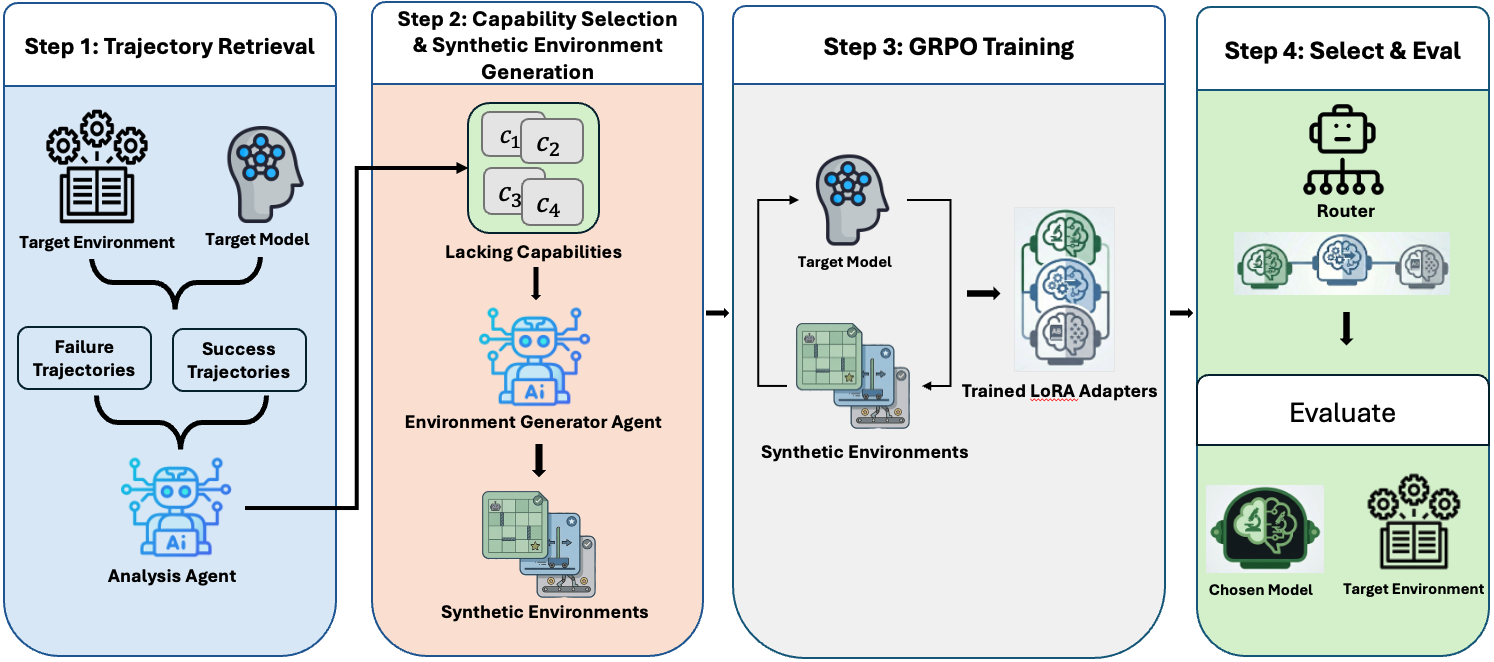
\includegraphics[width=0.9\textwidth]{figures/diagram_2.png}
    \caption{Overview of our framework. Starting from successful and failed trajectories collected in the target environment, an analysis agent identifies recurring missing capabilities through repeated contrastive analysis. For each retained capability, an environment-generation agent synthesizes a verifiable synthetic environment that preserves the target interface while isolating the missing behavior. We then train a separate capability-specific adapter in each synthetic environment and route between different adapters at inference time to improve performance on the original target environment. \textcolor{blue}{step 4 of figure is misleading fix}}
    \label{fig:framework_overview}
\end{figure*}

